\documentclass{article}
\usepackage{Description_of_methods}


\begin{document}

\hypersetup{
  pdftitle = {OverProt -- Supplementary information}
  % pdftitle = {OverProt -- Description of methods}
}

\title{Supplementary information for \\ ``OverProt: secondary structure consensus \\for protein families''}
% \title{OverProt -- Description of methods}

\author[1,2]{Adam Midlik}
\author[2,3,4]{Ivana Hutařová Vařeková}
\author[1,2]{Jan Hutař}
\author[1,2]{Aliaksei Chareshneu}
\author[4,*]{Karel Berka}
\author[1,2,*]{Radka Svobodová}

\affil[1]{CEITEC -- Central European Institute of Technology, Masaryk University, 625 00 Brno, Czech Republic}
\affil[2]{National Centre for Biomolecular Research, Faculty of Science, Masaryk University, 625 00 Brno, Czech Republic}
\affil[3]{Faculty of Informatics, Masaryk University, 602 00 Brno, Czech Republic}
\affil[4]{Department of Physical Chemistry, Faculty of Science, Palacký University, 771 46 Olomouc, Czech Republic}
\affil[*]{To whom correspondence should be addressed.}
\date{}  % omit date

\maketitle

\renewcommand{\contentsname}{Table of contents}
\tableofcontents
\clearpage



%%%%%%%%%%%%%%%%%%%%%%%%%%%%%%%%%%%%%%%%%%%%%%%%%%%%%%%%%%%%%%%%%%%%%%%%%%%%%%
%%%%%%%%%%%%%%%%%%%%%%%%%%%%%%%%%%%%%%%%%%%%%%%%%%%%%%%%%%%%%%%%%%%%%%%%%%%%%%
\section{Introduction}

OverProt is a tool for constructing and visualizing the secondary
structure consensus for protein families. The consensus produced by
OverProt can be used as a template for annotation of secondary structure
elements in protein families, e.g.~by SecStrAnnotator.

OverProt consists of three main parts: the main algorithm
\textbf{OverProt Core} constructs the secondary structure consensus,
\textbf{OverProt Viewer} visualizes the consensus, and \textbf{OverProt
Server} presents the results on the web and allows user-defined
computations.

The source code is freely available at \url{https://gitlab.com/midlik/overprot}.




%%%%%%%%%%%%%%%%%%%%%%%%%%%%%%%%%%%%%%%%%%%%%%%%%%%%%%%%%%%%%%%%%%%%%%%%%%%%%%
%%%%%%%%%%%%%%%%%%%%%%%%%%%%%%%%%%%%%%%%%%%%%%%%%%%%%%%%%%%%%%%%%%%%%%%%%%%%%%
\section{Terminology}

\begin{itemize}
  \item
    \textbf{Protein structure} -- a set of atoms with assigned 3D
    coordinates. A structure consists of one or more \textbf{chains}. A
    chain is a sequence of \textbf{residues}, each of which consists of the
    individual \textbf{atoms}. OverProt works with structures in
    \textbf{mmCIF format}. Structures deposited in the PDB 
    (\mycite{armstrong2020}{Armstrong \etal, 2020})
    are referenced by their PDB ID (e.g.~\code{1tqn}). OverProt follows the
    \emph{label*} numbering scheme when referencing chains and residues
    within a structure (i.e.~items \code{label\_asym\_id} and
    \code{label\_seq\_id} in the mmCIF file) -- this is in some cases
    different from the \emph{auth*} numbering scheme.
  \item
    \textbf{Protein domain} -- a part of protein structure, either a
    whole chain or a range (ranges) of residues in a chain. A domain is
    defined by the structure identifier (PDB ID), chain identifier, and one or more
    ranges of residues, e.g.~\code{1tqn,A,7:478} or
    \code{1n26,A,2:9,94:192}. Residue ranges include the start and end
    residue (e.g.~\code{5:8} means residues 5, 6, 7, 8).
  \item
    \textbf{Protein family} -- a set of protein domains with a reasonable
    structural similarity. The set can be provided by the user or it can
    be defined based on the CATH database (\mycite{sillitoe2021}{Sillitoe \etal, 2021}), 
    in which case the family (\emph{CATH superfamily}) is identified by its CATH ID
    (e.g.~\code{1.10.630.10}) and domains are identified by CATH domain
    ID (e.g.~\code{1tqnA00}).
  \item
    \textbf{Secondary structure element (SSE)} -- a section of a protein
    chain with some secondary structure pattern. OverProt focuses on two
    key types of SSEs -- \textbf{helices} (H) and \textbf{β-strands} (E). Each
    SSE within a protein structure can be identified by its chain
    identifier, start (index of its first residue), end (index of its last
    residue), and type (H/E). For comparing SSEs, it is convenient to simplify
    an SSE to a line segment (i.e.~3D coordinates of the start and end
    point).\\
    The term β-connectivity refers to the way in which the strands are
    connected: a \textbf{β-ladder} is a connection of two strands (realized 
    by hydrogen bonds) and can be either parallel or antiparallel; 
    a \textbf{β-sheet} is a set of
    strands which are connected by β-ladders (a connected component).\\
    This model is kept as simple as possible (different helix types
    (\(\alpha\), \(3_{10}\), \(\pi\)) are not distinguished; other SSE
    type (loops, turns) are not taken into account). Secondary structure
    assignment (detection of SSEs) is performed by
    \textbf{SecStrAnnotator}, more details can be found in its original paper 
    (\mycite{midlik2019}{Midlik \etal, 2019}).\\
    We will sometimes use the term \textbf{base SSEs} to distinguish SSEs from consensus SSEs.
  \item
    \textbf{Consensus SSE} -- a set of equivalent SSEs from different
    family members. 
  \item
    \textbf{Secondary structure consensus} -- a set of consensus SSEs
    with a given order and β-connectivity.
\end{itemize}




%%%%%%%%%%%%%%%%%%%%%%%%%%%%%%%%%%%%%%%%%%%%%%%%%%%%%%%%%%%%%%%%%%%%%%%%%%%%%%
%%%%%%%%%%%%%%%%%%%%%%%%%%%%%%%%%%%%%%%%%%%%%%%%%%%%%%%%%%%%%%%%%%%%%%%%%%%%%%
\section{Methods -- OverProt Core}

\textbf{OverProt Core} is an algorithm that constructs the secondary
structure consensus for a given protein family. The algorithm proceeds
in several steps. 
(In the following text, \code{--xx} refers to a command-line option of \path{overprot.py},
\code{[xx]yy} refers to a setting yy in section xx in the configuration file (\path{overprot-config.ini}).)



%%%%%%%%%%%%%%%%%%%%%%%%%%%%%%%%%%%%%%%%%%%%%%%%%%%%%%%%%%%%%%%%%%%%%%%%%%%%
\subsection{Preparation}

\begin{itemize}
  \item
    The list of domains for the family is downloaded from PDBe API
    \path{https://www.ebi.ac.uk/pdbe/api/mappings/{family_id}} 
    (if not already given by \code{--domains}).
  \item
    Select sample: If \code{--sample\_size} is smaller that the number of domains, 
    a random subset of the domain list is selected.\\
    The family may contain multiple domains from the same PDB entry. If 
    \code{[sample\_selec{\allowbreak}tion]{\allowbreak}unique\_pdb} is \code{True}, 
    then these are treated as duplicates and only one of them is selected 
    (the first in alphabetical order).
  \item
    Download structures: The structures of listed domains are downloaded
    in mmCIF format; the domains are cut out from the structures and saved in
    separate files. The sources of structures are given by
    \code{-\/-structure\_source} and
    \code{{[}download{]}structure\_sources}. The structures are also converted 
    to the PDB format for later steps (namely, for alignment by program MAPSCI). 
    The download step is performed by an auxiliary program \code{StructureCutter} 
    written in C\# (a part of the OverProt project).
  \end{itemize}
  


%%%%%%%%%%%%%%%%%%%%%%%%%%%%%%%%%%%%%%%%%%%%%%%%%%%%%%%%%%%%%%%%%%%%%%%%%%%%
\subsection{Structural alignment}

Multiple structure alignment is performed in 2 steps:

\begin{itemize}
\item
  Program MAPSCI (\mycite{ilinkin2010}{Ilinkin \etal, 2020}) is used to calculate a
  consensus structure (\path{mapsci/consensus.cif}).
  For performance reasons, at most 100 domains are selected for this
  calculation (in a quasi-random way, i.e.~for the same family it selects 
  the same subset every time).\\
  To reduce indeterminism and ease later visualization, the consensus
  structure is centered to the origin (0, 0, 0), rotated so that its PCA
  (principal component analysis)
  components are aligned to the XYZ axes (``the structure is laid
  flat''), and flipped in a consistent way (roughly so that the start and 
  the end of the chain are more in front, and the chain goes from left-top 
  to right-bottom).\\
  In general, MAPSCI produces a reasonable consensus structure, but the
  alignment of the individual domains is often poor, so the
  following re-alignment step is necessary.
\item
  In the re-alignment step, all domains are structurally aligned onto the
  MAPSCI consensus structure via \code{cealign} algorithm 
  (\mycite{shindyalov1998}{Shindyalov and Bourne, 1998})
  provided in PyMOL module (\mycite{schrodinger}{Schrödinger, LLC.}) version 2.3.0. 
  In rare cases \code{cealign} fails (when the domains are too short) -- 
  in such cases a simple internal algorithm is used instead (theoretically 
  inefficient and not allowing gaps, but sufficient for these
  very short domains).
\end{itemize}



%%%%%%%%%%%%%%%%%%%%%%%%%%%%%%%%%%%%%%%%%%%%%%%%%%%%%%%%%%%%%%%%%%%%%%%%%%%%
\subsection{Secondary structure assignment}

The SSEs in each domain are detected by \code{SecStrAnnotator} 
(\mycite{midlik2019}{Midlik \etal, 2019}, \mycite{midlik2021}{2021}) 
with options ~\code{-\/-onlyssa} ~\code{-\/-verbose} ~\code{-\/-batch}.



%%%%%%%%%%%%%%%%%%%%%%%%%%%%%%%%%%%%%%%%%%%%%%%%%%%%%%%%%%%%%%%%%%%%%%%%%%%%
\subsection{Guide tree}

The domains are clustered by agglomerative clustering to produce a \textbf{guide
tree}. The algorithm starts with a set of structures. It finds the two 
most similar structures and merges them into a new structure. This is then
repeated until we end up with a single structure corresponding
to the tree root.

This agglomerative algorithm can be expressed by the following
pseudocode:

\begin{codeblock}
    Workset = { the structures of all input domains }  
    while |Workset| > 1:  
        A, B = two nearest structures in Workset
        C = merge_structures(A, B)  
        Children of C = {A, B}
        Workset = Workset - {A, B} ∪ {C}
\end{codeblock}

At the end, \code{Workset} will only contain one structure,
which is the tree root. The topology of the tree will be defined by
\code{Children}. An example is shown in Figure \ref{fig:guide_tree}.

\begin{figure}[h!]
  \centering{
    \begin{codeblock}
                      A────────────┐
                                   │
                      B────┐       ├ABC──────┐
                           ├BC─────┘         │
                      C────┘                 ├ABCDE
                                             │
                      D────────┐             │
                               ├DE───────────┘
                      E────────┘
    \end{codeblock}
  }
  \caption{An example of the guide tree construction. 5 structures were initially in \code{Workset}.
  B+C were merged into BC, then D+E into DE, then A+BC into ABC, and finally ABC+DE into ABCDE.}
  \label{fig:guide_tree}
\end{figure}

The details of the algorithm are described in Appendix \ref{sec:appendix_ws_distance} 
(distance function, which determines the nearest structures) 
and \ref{sec:appendix_ws_merging} (operation \code{merge\_structures}).



%%%%%%%%%%%%%%%%%%%%%%%%%%%%%%%%%%%%%%%%%%%%%%%%%%%%%%%%%%%%%%%%%%%%%%%%%%%%
\subsection{Merging}
\label{sec:merging}

This step is the core of the consensus generation algorithm. As an input, we
have a set of \emph{k}~protein domains. Each domain is simplified to a
sequence of SSEs (defined by their type, line segment, etc.). 
The required output is a clustering of all input SSEs (see Figure \ref{fig:clusters}).

\begin{figure}[h!]
  \centering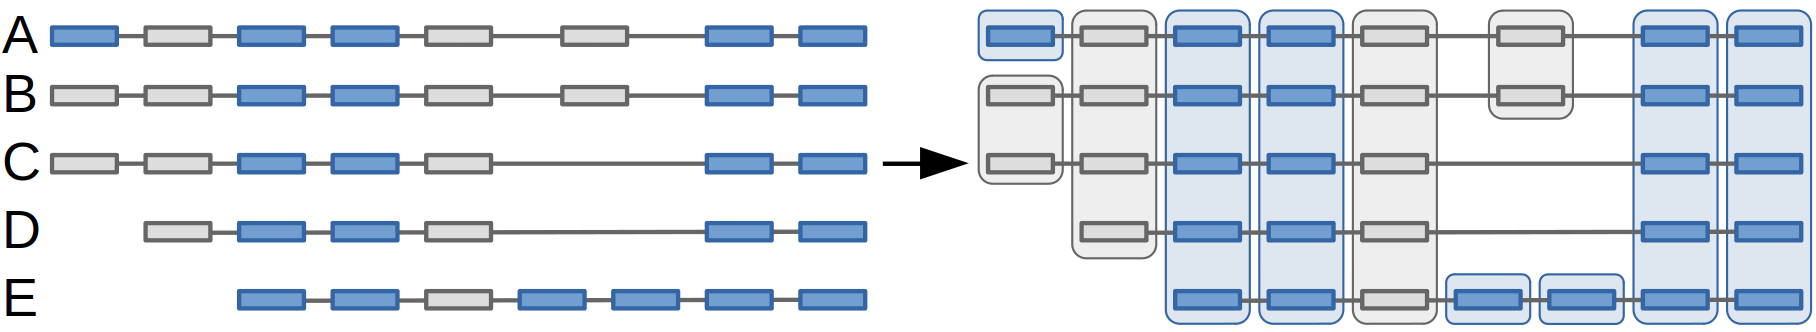
\includegraphics[width=\linewidth]{figures/clusters.png}
  \caption{An example of 5 domains simplified to a sequence of base SSEs 
  (gray = helix, blue = strand) and their clustering into 11 clusters.}
  \label{fig:clusters}
\end{figure}

However, the clustering must fulfil these constraints:

\begin{enumerate}
\def\labelenumi{\arabic{enumi}.}
% \tightlist
\item
  Each cluster can contain only elements of the same type (only helices
  or only strands).
\item
  A cluster must not contain more than one element from the same protein
  domain.
\item
  There must be a partial order of the clusters. This constraint can be formalized as:
  \begin{itemize}
    \item
      Base SSE \(x\) precedes base SSE \(y\) (written \(x \rightarrow y\)) if they
      are from the same protein domain and \(x\) goes before \(y\) in the sequence.
    \item
      Cluster \(P\) directly precedes cluster \(Q\) (\(P \Rightarrow Q\)) if there
      exist SSEs \(x \in P, y \in Q\) such that \(x \rightarrow y\).
    \item
      Cluster \(P\) precedes cluster \(Q\) (\(P \rightarrow Q\)) if there
      exists a sequence of clusters \(P \Rightarrow R_1 \Rightarrow ... 
      \Rightarrow R_n = Q\) where \(n \geq 1\) (in other words, \(\rightarrow\) 
      is the transitive closure of \(\Rightarrow\)).
    \item
      There must be no cluster \(P\), such that \(P \rightarrow P\).
  \end{itemize}
\end{enumerate}

Note: The order of some clusters may be undefined (i.e.~neither 
\(P \rightarrow Q\) nor \(Q \rightarrow P\)) if they contain no SSEs 
from the same domain. Therefore \(\rightarrow\) is a partial order on the clusters (not a total order).
We represent the order by a directed acyclic graph (DAG) (see Figure \ref{fig:dag_example}).

\begin{figure}[h!]
  \centering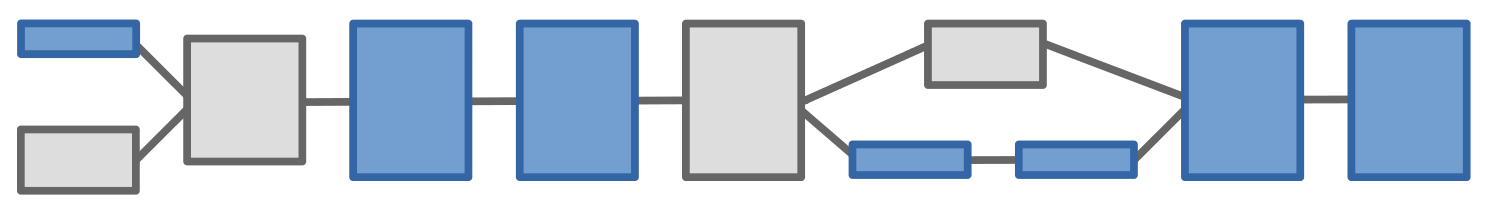
\includegraphics[width=0.6\linewidth]{figures/dag_ABCDE.png}
  \caption{An example of a DAG representing clusters of SSEs from Figure \ref{fig:clusters}. 
  The height of each rectangle shows the weight of the cluster (the number of base SSEs in the cluster).
  The color shows the cluster type (gray = helix, blue = strand).
  The direction of the edges is implicit (left to right).
  The egdes that can be inferred from transitivity are not shown 
  (i.e.~we show only the transitive reduction (Hasse diagram)). }
  \label{fig:dag_example}
\end{figure}

The merging step follows the guide tree. First, each guide tree leaf is
populated with the DAG of SSEs of the respective domain. 
In each internal node, the DAGs from the two children nodes are matched together and merged. 
The root then contains the consensus SSEs of the whole family (see Figure \ref{fig:dag_merging}). 

\begin{figure}[h!]
  \centering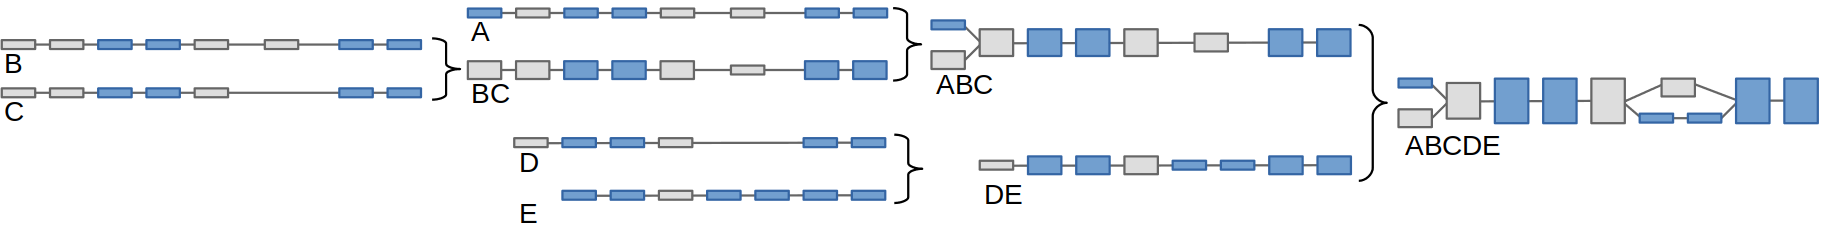
\includegraphics[width=\linewidth]{figures/dag_merging.png}
  \caption{The process of merging 5 DAGs based on the guide tree from Figure \ref{fig:guide_tree}.}
  \label{fig:dag_merging}
\end{figure}

The matching and merging of two SSE DAGs is in principle similar to matching
and merging of two weighted structures. 
The best matching is also found by dynamic programming.
However, it is more complicated here because 
1) SSEs of different type cannot be matched (this can cause the
branching in the resulting DAG), 
and 2) the dynamic programming algorithm is not as straightforward 
for matching DAGs as it is for matching sequences.
More details are provided in Appendix \ref{sec:appendix_matching_dags}.

The β-connectivity is not directly considered in the merging algorithm 
(though it is included in the distance function for DAG matching).
Therefore it is necessary to determine the β\nobreakdash-connectivity of the resulting clusters 
based on the β-connectivity of the base SSEs.

A β-ladder \(PQo\) (connecting strand clusters \(P\) and \(Q\) with orientation \(o\) (parallel/antiparallel)) 
is included in the resulting consensus if
  \[  \frac { n_{PQo} } { \min{\{n_P, n_Q\}} } \geq 0.5  \]
where \(n_P\) is the number of strands in cluster \(P\), 
\(n_Q\) is the number of strands in cluster \(Q\),
and \(n_{PQo}\) is the number of base ladders connecting a base strand in \(P\) to a base strand in \(Q\)
with orientation \(o\) (see Figure \ref{fig:dag_ladders}).

\begin{figure}[h!]
  \centering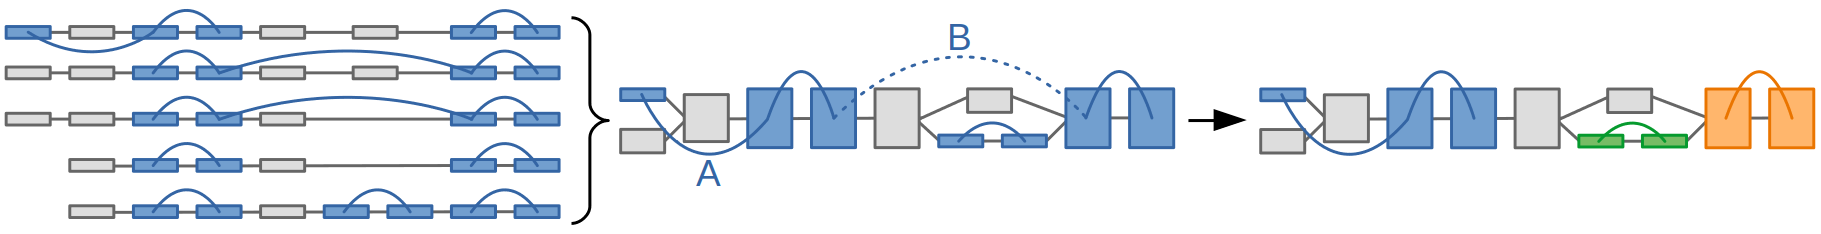
\includegraphics[width=\linewidth]{figures/dag_ladders.png}
  \caption{Merging β-ladders from 5 domains. 
  Lower arcs show parallel, upper arcs antiparallel ladders.
  Ladder A is included because \( n_{PQo} / \min{\{n_P, n_Q\}} = 1 / \min{\{1, 5\}} = 1 \geq 0.5\).
  Ladder B is not included because \( n_{PQo} / \min{\{n_P, n_Q\}} = 2 / \min{\{5, 5\}} = 0.4 < 0.5\).
  The rightmost column shows the separation of the consensus strands into sheets (connected components).}
  \label{fig:dag_ladders}
\end{figure}

After the clustering, a variety of statistics are computed for each consensus SSE and saved in \path{results/consensus.sses.json}: 
\begin{itemize}
  \item
    Occurrence -- the number of domains that contain this SSE, 
    divided by the total number of domains in the family. 
    In the previous example, the first strand occurs in 1 out of 5 domains; 
    thus its occurrence is 0.2 or 20\%.
  \item
    Average length -- measured as the number of residues.
  \item
    Average line segment -- the average start and end point in 3D.
  \item
    3D variability -- the variance of the start and end point.
\end{itemize}

Each consensus SSE also gets a unique label (containing its type and sequential number, e.g. E0, H1, H2...) and color.

%%%%%%%%%%%%%%%%%%%%%%%%%%%%%%%%%%%%%%%%%%%%%%%%%%%%%%%%%%%%%%%%%%%%%%%%%%%%
\subsection{Annotation}

In this optional step, the generated SSE consensus is used
as an annotation template for SecStrAnnotator, and all family members are
annotated. Before the annotation, the SSEs with low occurrence
(\textless{} 5\%) are removed, which dramatically reduces the running
time of SecStrAnnotator. SecStrAnnotator is run with these options:
\code{-\/-ssa\ file} ~\code{-\/-align\ none}
~\code{-\/-metrictype~3} ~\code{-\/-fallback\ 30}
~\code{-\/-unannotated}. 
Metric type 3 must be used because the default metric requires 
residue numbers for each SSE, but these are not available for the consensus SSEs. 
Option \code{-\/-unannotated} includes also the unannotated SSEs in the resulting annotation files, 
with labels prefixed by underscore (e.g. \code{\_H0}).



%%%%%%%%%%%%%%%%%%%%%%%%%%%%%%%%%%%%%%%%%%%%%%%%%%%%%%%%%%%%%%%%%%%%%%%%%%%%
\subsection{Visualization}

The generated SSE consensus is visualized by several SVG diagrams with
different settings and \path{diagram.json} file is produced, which
will be used for interactive visualization by OverProt Viewer. 
A PyMOL session (.pse) is created, with the MAPSCI consensus structure 
shown as ribbon and the consensus SSEs shown as cylinders and arrows.
The width of each cylinder/arrow shows the occurrence of the corresponding helix/strand.
A PNG image is also rendered from the session. 
A session with all domains and their SSEs is
generated if \code{[visual{\allowbreak}ization]{\allowbreak}create\_multi\_session} is
\code{True} (very slow, not recommended for larger families).



%%%%%%%%%%%%%%%%%%%%%%%%%%%%%%%%%%%%%%%%%%%%%%%%%%%%%%%%%%%%%%%%%%%%%%%%%%%%
\subsection{Execution}

OverProt Core is implemented mostly in Python3 
and designed to run in the Linux environment (tested on Ubuntu 20.04).
On the other operating systems, it can be run in Docker.
Before the first execution, the dependencies must be installed:

\begin{codeblock}
  sh install.sh --clean
\end{codeblock}

All steps of the algorithm are combined in \path{overprot.py}. 
It is run in a Python virtual environment. 
Its arguments are the CATH family ID and the output directory:

\begin{codeblock}
  . venv/bin/activate
  python overprot.py --help
  python overprot.py 1.10.630.10 data/cyp/
\end{codeblock}

Multiple families can be processed in parallel using \path{overprot_multifamily.py}. 
Its arguments are the family list and the output directory:

\begin{codeblock}
  . venv/bin/activate
  python overprot_multifamily.py --help
  python overprot_multifamily.py data/families.txt data/multifamily/
\end{codeblock}

More details can be found in the \code{README.md} files 
in the project repository.


%%%%%%%%%%%%%%%%%%%%%%%%%%%%%%%%%%%%%%%%%%%%%%%%%%%%%%%%%%%%%%%%%%%%%%%%%%%%%%
%%%%%%%%%%%%%%%%%%%%%%%%%%%%%%%%%%%%%%%%%%%%%%%%%%%%%%%%%%%%%%%%%%%%%%%%%%%%%%
\section{Interactive visualization by OverProt Viewer}

\textbf{OverProt Viewer} is a web component for interactive
visualization of the SSE consensus. Its input is the preprocessed
\path{diagram.json} file. It is implemented in TypeScript with D3.js.

OverProt Viewer shows each consensus SSE as a rectangle or an oval, whose height 
corresponds to its occurrence 
and width corresponds to its average length (number of residues). 
Strands from the same β-sheet are shown in the same color; helices are shown in gray. 
Connections of the strands in a β-sheet are shown by arcs 
(lower arcs -- parallel, upper arcs -- antiparallel). 
Hovering over an SSE shape shows the SSE details (see Figure \ref{fig:overprot_viewer}).

\begin{figure}[h!]
  \centering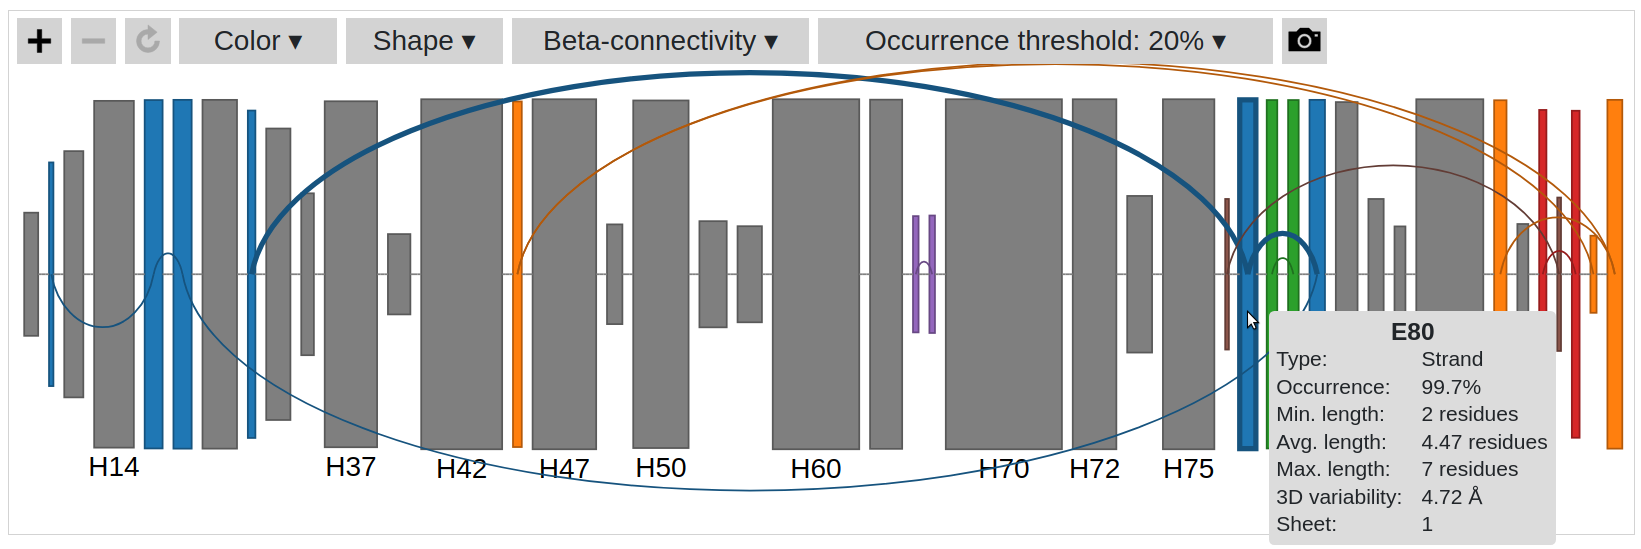
\includegraphics[width=\linewidth]{figures/overprot_viewer.png}
  \caption{OverProt Viewer showing the secondary structure consensus for CATH family 1.10.630.10 (Cytochrome P450).}
  \label{fig:overprot_viewer}
\end{figure}

Visualization options include: 

\begin{itemize}
  \item
    Color:
    \begin{denseitemize}     \item
        Uniform -- Show all SSEs in the same color.
      \item
        Type -- Show β-strands in blue, helices in gray.
      \item
        Sheet -- Assign the same color to all β-strands from the same β-sheet; show helices in gray.
      \item
        Variability -- The 3D variability measures the standard deviation of the SSE start and end point coordinates. 
        Low values (dark) indicate conserved SSE position, high values (bright) indicate variable SSE position.
      \item
        Rainbow -- Standard rainbow coloring from N-terminus (blue) to C-terminus (red).
    \end{denseitemize}
    
  \item
  Shape:
  \begin{denseitemize}
    \item
      Rectangle -- Show the SSEs as rectangles. The height of the rectangle indicates its occurrence; the width indicates its average length (number of residues).
    \item
      SymCDF -- The cumulative distribution function (CDF) describes the statistical distribution of the SSE length. 
      The SymCDF shape consists of four symmetrical copies of the CDF; the bottom right quarter is the classical CDF.
      The widest part of the shape corresponds to the maximum length, 
      the narrowest to the minimum length, the height corresponds to the occurrence. 
  \end{denseitemize}
  
  \item
    Beta-connectivity:
    \begin{denseitemize}
      \item
        On -- The beta-connectivity shows how β-strands are connected to each other in β-sheets.
        The lower arcs indicate parallel ladders;
        the upper arcs indicate antiparallel ladders.
      \item
        Off -- The beta-connectivity arcs are hidden.
    \end{denseitemize}
    
  \item
  Occurrence threshold:
  \begin{denseitemize}
    \item
      Hides the SSEs with occurrence lower than the specified threshold. Can be set to any number from 0\% to 100\%.
  \end{denseitemize}
\end{itemize}

OverProt Viewer can be set to dispatch and listen to HTML events. 
When an SSE is hovered over or clicked, the viewer dispatches an event 
(\code{PDB.overprot.hover} or \code{PDB.overprot.\allowbreak select}). 
The information about the selected elements is included in \code{event.detail}.
Conversely, the viewer handles the incoming events (\code{PDB.overprot.do.hover} 
or \code{PDB.overprot.\allowbreak do.\allowbreak select}) by highlighting the selected elements. 
This allows interactivity across several web components, as demonstrated by 
the integrated view in the OverProt web 
(\url{https://overprot.ncbr.muni.cz/domain_view?family_id=1.10.630.10&domain_id=1jfbA00})
-- hovering over an SSE in any of the three components (OverProt Viewer, 
interactive 2DProts (\mycite{hutarova2021}{Hutařová \etal, 2021}), 
MolStar Viewer (\mycite{sehnal2021}{Sehnal \etal, 2021})) highlights it in all three.





%%%%%%%%%%%%%%%%%%%%%%%%%%%%%%%%%%%%%%%%%%%%%%%%%%%%%%%%%%%%%%%%%%%%%%%%%%%%%%
%%%%%%%%%%%%%%%%%%%%%%%%%%%%%%%%%%%%%%%%%%%%%%%%%%%%%%%%%%%%%%%%%%%%%%%%%%%%%%
\section{Data computation for OverProt Server}

\textbf{OverProt Server} provides precomputed SSE consensuses (database)
and runs the OverProt Core algorithm for user-defined sets of domains (jobs). 
OverProt Server is implemented using Python (Flask), Gunicorn, Redis Queue, Nginx, and Docker.
A running instance is available at \url{https://overprot.ncbr.muni.cz}.


The database is constructed in this way:

\begin{itemize}
\item
  Retrieve the current list of families from CATH
  (\url{http://download.cathdb.info/cath/releases/latest-release/cath-classification-data/cath-superfamily-list.txt}).
  The list currently contains 6631 families, out of which 64 are empty
  families (January 2022).
\item
  Retrieve the domain lists for each family, including chains and
  residue ranges, from PDBe API
  (\path{https://www.ebi.ac.uk/pdbe/api/mappings/{family_id}}). This is
  currently over 470k domains in total (January 2022).
\item
  Remove duplicates (i.e.~multiple domains from the same PDB entry).
  The number of domains without duplicates is currently over 200k (January 2022).
\item
  Apply the OverProt Core algorithm to each family.
\end{itemize}

The whole process is realized by:

\begin{codeblock}
  . venv/bin/activate
  python  overprot_multifamily.py  --download_family_list_by_size \
      --config working_scripts/overprot-config-overprotserverdb.ini \
      --collect  -  $UPDATE_DIRECTORY                                                           $
\end{codeblock}



%%%%%%%%%%%%%%%%%%%%%%%%%%%%%%%%%%%%%%%%%%%%%%%%%%%%%%%%%%%%%%%%%%%%%%%%%%%%%%
%%%%%%%%%%%%%%%%%%%%%%%%%%%%%%%%%%%%%%%%%%%%%%%%%%%%%%%%%%%%%%%%%%%%%%%%%%%%%%
\section{Appendix} 
\label{sec:appendix}



%%%%%%%%%%%%%%%%%%%%%%%%%%%%%%%%%%%%%%%%%%%%%%%%%%%%%%%%%%%%%%%%%%%%%%%%%%%%
\subsection{Distance function for two weighted structures}
\label{sec:appendix_ws_distance}

To be able to compare the real structures of the input domains as well as the artificial 
structures created by merging, we use the concept of a weighted structure. 
A weighted structure is a sequence of points (C-alpha coordinates)
where each point has its relative weight. 
In any real structure, all relative weights are equal to 1, 
but merging can create points with smaller relative weights.
The absolute weight of a weighted structure is simply the number of the real structures 
that have been merged to form this weighted structure.

Formally, a weighted structure \(A\) is a tuple
\( (n^A, \mathbf{R}^A, \mathbf{W}^A, k^A) \) where \(n^A\) is the length
of the weighted structure (number of points), \(\mathbf{R}^A\) is the
matrix of their coordinates (\(n^A \times 3\)), \(\mathbf{W}^A\) is the
vector of their relative weights \(\in (0,1]\), and \(k^A\) is the
absolute weight of \(A\). Example of a weighted structure:
  \[
    n^A = 4 \quad
    \mathbf{R}^A = \begin{bmatrix}-1.1&-2.9&0.1&0.4\\0.0&1.1&0.9&-2.7\\5.2&2.1&0.0&0.8\end{bmatrix} \quad
    \mathbf{W}^A = \begin{bmatrix}1&0.5&0.8&1\end{bmatrix} \quad
    k^A = 10
  \]

\(\mathbf{r}^A_i\) and \(w^A_i\) will refer to \(i\)-th column of
\(\mathbf{R}^A\) and \(\mathbf{W}^A\).

A protein domain can be converted into a weighted structure as follows:
\(n\) is the number of residues, \(\mathbf{r}^A_i\) are the coordinates of the
C-alpha atom of \(i\)-th residue, \(w^A_i\) is 1, and \(k^A\) is 1.

The distance function \(d\) is defined for two weighted points:
  \[
    d \left( (\mathbf{r}^A_i, w^A_i), (\mathbf{r}^B_j, w^B_j) \right) 
    = \left( 1 - e^{-\lVert \mathbf{r}^A_i-\mathbf{r}^B_j \rVert / R_0} \right) \cdot \min\{ w^A_i, w^B_j \} + \frac{1}{2} \lvert w^A_i-w^B_j \rvert
  \]

The parameter \(R_0\) was set to 10~\AA.

In case that one of the weighted points is undefined (\(\bot\)), \(d\)
is still defined:
  \[
    d \left( (\mathbf{r}^A_i, w^A_i), \bot \right) = \frac{1}{2} w^A_i \qquad 
    d \left( \bot, (\mathbf{r}^B_j, w^B_j) \right) = \frac{1}{2} w^B_j
  \]

(Notes: Distance \(d\) is not the Euclidean distance of the two points.
\(d \in [0,1)\).)

A matching (or alignment) of two weighted structures \(A\), \(B\) is a sequence of
pairs \([(p_1, q_1), (p_2, q_2), \allowbreak ...\allowbreak(p_n, q_n)]\), 
where \(p_i\) and \(q_i\) are indices of the points of \(A\) and \(B\).
Indices must be increasing and must include each index exactly once for
both \(A\) and \(B\). Value \(\bot\) means that a particular point was
not matched. Example of a valid matching for \(n^A = 4, n^B = 5\):
  \[  [(1, 1),\ (2, \bot),\ (3, 2),\ (4, 3),\ (\bot, 4),\ (\bot, 5)]  \]
  
The distance function \(D\) for two weighted structures \(A\) and \(B\) with a given matching \(M\) is defined:
  \[  D(A, B, M) = \sum\limits_{(p, q) \in M}{d \left( (\mathbf{r}^A_{p}, w^A_{p}), (\mathbf{r}^B_{q}, w^B_{q}) \right)}  \]

  The distance function \(D^*\) of two weighted structures \(A\) and \(B\) is then:
  \[  D^*(A, B) = D(A, B, M^*)  \]
where \(M^*\) is the best matching of \(A\) and \(B\), i.e.~the matching which minimizes \(D(A, B, M^*)\).

The best matching can be found by dynamic programming. 
For this, the distance function \(d\) is converted into the score function \(s\):
  \[
    s \left( (\mathbf{r}^A_i, w^A_i), (\mathbf{r}^B_j, w^B_j) \right) 
    = \frac{1}{2} w^A_i + \frac{1}{2} w^B_j - d \left( (\mathbf{r}^A_i, w^A_i), (\mathbf{r}^B_j, w^B_j) \right)
  \]
  \[
    s \left( (\mathbf{r}^A_i, w^A_i), \bot \right) = 0 \qquad 
    s \left( \bot, (\mathbf{r}^B_j, w^B_j) \right) = 0
  \]

Similarly, \(D\) is converted into the total score function \(S\):
  \[
    S(A, B, M) 
    = \sum\limits_{(p, q) \in M}{s \left( (\mathbf{r}^A_{p}, w^A_{p}), (\mathbf{r}^B_{q}, w^B_{q}) \right)}
    = \frac{1}{2} \sum\limits_{i=1}^{n^A}{w^A_i} + \frac{1}{2} \sum\limits_{j=1}^{n^B}{w^B_j} - D(A, B, M)
  \]

From this equation, it can be seen that maximizing \(S\) by dynamic
programming also minimizes \(D\). (This dynamic programming algorithm is in principle
very similar to the well-known Needleman-Wunsch algorithm for aligning sequences 
(\mycite{needleman1970}{Needleman and Wunsch, 1970}), 
but it differs in the score function it uses.)

\paragraph{Notes:} 
The distance function \(D^*\) is inspired by the edit distance for 
comparing two strings. It basically measures how much we have to edit \(A\) 
(move/insert/delete points) to transform it into \(B\). 
Thanks to this design, \(D^*\) is a metric 
(i.e.~\(D^*(A,A) = 0\), \(D^*(A,B) = D^*(B,A)\), and
\(D^*(A,B) + D^*(B,C) \geq D^*(A,C)\) for any weighted structures
\(A, B, C\)).

When finding the two nearest items in the workset, it is not
necessary to calculate the distance \(D^*\) for every pair of items --
there are specialized data structures that can significantly decrease
the number of distance calculations. We use a non-standard structure
NN-tree (nearest neighbor tree). In some larger protein families, this
can reduce the number of distance computations to less than 20\%. 
(Standard structures like GH-tree, M-tree, etc. either miss some of
the necessary operations (insert, delete) or perform worse than NN-tree
for this particular application.) This is only possible because \(D^*\) 
is a metric.




%%%%%%%%%%%%%%%%%%%%%%%%%%%%%%%%%%%%%%%%%%%%%%%%%%%%%%%%%%%%%%%%%%%%%%%%%%%%
\subsection{Merging two weighted structures}
\label{sec:appendix_ws_merging}

Having two weighted structures \(A, B\) and their best matching
\(M^* = [(p_1, q_1), ... (p_n, q_n)]\), we can define 
operation \(merge\_structures\) as follows:
  \[  merge\_structures(A, B) = C = (n^C, \mathbf{R}^C, \mathbf{W}^C, k^C)  \]
  \[  n^C = n  \]
  \[  \mathbf{r}^C_i = \frac {\mathbf{r}^A_{p_i} w^A_{p_i} k^A + \mathbf{r}^B_{q_i} w^B_{q_i} k^B} {w^A_{p_i} k^A + w^B_{q_i} k^B}  \]
  \[  w^C_i = w^A_{p_i} k^A + w^B_{q_i} k^B  \]
  \[  k^C = k^A + k^B  \]
(If \(p_i=\bot\), the values can be calculated by setting
\(w^A_{p_i} = 0\), thus simplifying to
\(\mathbf{r}^C_i = \mathbf{r}^B_{q_i}, w^C_i = w^B_{q_i}\). Similarly for \(q_i=\bot\).)




\subsection{Matching two SSE directed acyclic graphs (DAGs)}
\label{sec:appendix_matching_dags}

The distance function \(d\) for two SSEs \(P\) and \(Q\) is defined 
as the sum of Euclidean distances between their start points and between their end points:
  \[  d(P, Q) = \lVert \mathbf{u}_P - \mathbf{u}_Q \rVert + \lVert \mathbf{v}_P - \mathbf{v}_Q \rVert  \]
where \(\mathbf{u}_P, \mathbf{v}_P\) is the start and end point of SSE \(P\), 
\(\mathbf{u}_Q, \mathbf{v}_Q\) is the start and end point of SSE \(Q\).

The score function \(s\) is then defined:
  \[
    s(P, Q) = \begin{cases}
                SR(d(P, Q)) \quad & \mathrm{if}\ P, Q\ \mathrm{are\ of\ the\ same\ type\ (helix/strand)} \\
                0           \quad & \mathrm{otherwise}
              \end{cases}
  \]
where \(SR\) is the ``smoothed ramp'' function, which is basically 
a smooth, strictly decreasing version of the function \(y = \max\{0, 1 - x/d_0\} \). \\
\(SR\) is defined by the implicit equation 
\(  d_0 (1 - \alpha) y^2 + (x + d_0 (2\alpha - 1)) y - d_0 \alpha = 0  \).
When solving this quadratic equation, the greater root is selected.
The parameters were set to \(d_0 = 30\)~\AA\ and \(\alpha = 0.01\).

The distance function \(d\) and the score function \(s\) can be easily 
extended from base SSEs to consensus SSEs. 
For a consensus SSE \(P\), the point \(\mathbf{u}_P\) is simply 
the arithmetic mean of \(\mathbf{u}\) of all base SSEs included in \(P\).
Similarly for \(\mathbf{v}_P\).

However, it will be useful to define the weight of a consensus SSE \(P\) (\(w_P\)) 
as the number of base SSEs included in \(P\).
Similarly, we will define the weights of the consensus β-ladders:
\(w_{PQp}\) is the number of parallel ladders connecting 
a base strand in \(P\) to a base strand in \(Q\),
\(w_{PQa}\) is the number of antiparallel ladders connecting 
a base strand in \(P\) to a base strand in \(Q\). 
(Base SSEs/ladders can be understood as consensus SSEs/ladders with weight 1.)

In order to reflect the β-connectivity in the score function, 
the ``ladder correction'' is applied to the strands:
  \[  s_\mathrm{corr}(P_i, Q_j) = \frac{1}{2} \left( s(P_i, Q_j) + \sum_k \sum_l (\alpha_{ijkl} + \beta_{ijkl}) s(P_k, Q_l) \right)  \]
where \(P_i, P_k\) are strands in the first matched DAG, 
\(Q_j, Q_l\) are strands in the second matched DAG, 
and the coefficients \(\alpha_{ijkl}, \beta_{ijkl}\) 
maximize the value of \(s_\mathrm{corr}(P_i, Q_j)\)
while fulfilling the following constraints:
  \[  \alpha_{ijkl} \geq 0 \qquad  \beta_{ijkl} \geq 0  \]
  \[  \sum_k \sum_l (\alpha_{ijkl} + \beta_{ijkl}) \leq 1  \]
  \[  \sum_l \alpha_{ijkl} \leq \frac{w_{P_i P_k a}}{w_{P_i}}  \qquad  \sum_l \beta{ijkl} \leq \frac{w_{P_i P_k p}}{w_{P_i}}  \]
  \[  \sum_k \alpha_{ijkl} \leq \frac{w_{Q_j Q_l a}}{w_{Q_j}}  \qquad  \sum_k \beta{ijkl} \leq \frac{w_{Q_j Q_l p}}{w_{Q_j}}  \]

For each pair \(P_i, Q_j\), the values of coefficients \(\alpha_{ijkl}, \beta_{ijkl}\) 
are determined by a greedy algorithm (i.e.~first assigning the greatest possible value 
to the coefficients corresponding to the highest \(s(P_k, Q_l)\), then the second highest, etc.). 

For helices, no ``ladder correction'' is necessary, so \(s_\mathrm{corr}(P_i, Q_j) = s(P_i, Q_j)\).

A matching of two SSE DAGs \(\graph{G}, \graph{H}\) is a set of pairs 
\(M = \{(P_1, Q_1), (P_2, Q_2), ... (P_n, Q_n)\}\),
where \(P_i \in V(\graph{G}), Q_j \in V(\graph{H})\), fulfilling these conditions:

\begin{denseitemize}     
  \item Each vertex is matched at most once: \(\forall i, j: P_i \neq P_j \Leftrightarrow Q_i \neq Q_j\)
  \item Only vertices of the same type are matched: \(\forall i: \mathrm{type}(P_i) = \mathrm{type}(Q_i)\)
  \item No cycle is created: \(\nexists i, j: P_i \rightarrow P_j \wedge Q_j \rightarrow Q_i\)
\end{denseitemize}

The best matching \(M^*\) of DAGs \(\graph{G}, \graph{H}\) is the matching which maximizes 
the total score \(S\):
  \[  S(\graph{G}, \graph{H}, M^*) = \sum_{(P, Q) \in M^*} w_{P} w_{Q} s_\mathrm{corr}(P, Q)  \]
The corresponding best score is \(S^*\):
  \[  S^*(\graph{G}, \graph{H}) = S(\graph{G}, \graph{H}, M^*)  \]
The problem of finding the best matching and the best score 
for two DAGs \(\graph{G}, \graph{H}\) can be decomposed 
to smaller problems:
  \[ \begin{aligned}
    S^*(\graph{G}, \graph{H}) = \max\Big( & \{ S^*(\graph{G}-P, \graph{H}) \mid P \in \mathrm{sinks}(\graph{G}) \} \\
                                \cup\     & \{ S^*(\graph{G}, \graph{H}-Q) \mid Q \in \mathrm{sinks}(\graph{H}) \} \\
                                \cup\     & \{ S^*(\graph{G}-P, \graph{H}-Q) + w_{P} w_{Q} s_\mathrm{corr}(P, Q) \mid P \in \mathrm{sinks}(\graph{G}), Q \in \mathrm{sinks}(\graph{H}) \} \Big)  
  \end{aligned} \]
The trivial subproblems can be solved directly without decomposition: 
  \[  S^*(\graph{G}, \graph{K_0}) = S^*(\graph{K_0}, \graph{H}) = 0  \qquad \qquad \qquad  
      M^*(\graph{G}, \graph{K_0}) = M^*(\graph{K_0}, \graph{H}) = \{\}  
  \]
where \(\graph{K_0}\) is a graph with no vertices.

OverProt finds the best matching by a dynamic programming 
algorithm based on the described decomposition.

After the best matching is found, the matched pairs of vertices are merged. 
The resulting DAG contains the merged matched vertices 
plus the nonmatched vertices from the original DAGs \(\graph{G}, \graph{H}\).
The edges are merged accordingly, and transitive closure is applied.
If vertices \(P, Q\) are matched and merged into a vertex \(R\), then:
  \[  w_R = w_P + w_Q  \qquad\qquad
      \mathbf{u}_R = \frac{\mathbf{u}_P w_P + \mathbf{u}_Q w_Q}{w_P + w_Q}  \qquad\qquad
      \mathbf{v}_R = \frac{\mathbf{v}_P w_P + \mathbf{v}_Q w_Q}{w_P + w_Q}  
  \]



%%%%%%%%%%%%%%%%%%%%%%%%%%%%%%%%%%%%%%%%%%%%%%%%%%%%%%%%%%%%%%%%%%%%%%%%%%%%%%
%%%%%%%%%%%%%%%%%%%%%%%%%%%%%%%%%%%%%%%%%%%%%%%%%%%%%%%%%%%%%%%%%%%%%%%%%%%%%%
\section{References}

\myreference
{armstrong2020}
{Armstrong,D.R. \etal\ (2020) 
PDBe: improved findability of macromolecular structure data in the PDB. 
\emph{Nucleic Acids Res}, \textbf{48}, D335--D343.}
{https://doi.org/10.1093/nar/gkz990}

\myreference
{hutarova2021}
{Hutařová Vařeková,I. \etal\ (2021) 
2DProts: database of family-wide protein secondary structure diagrams. 
\emph{Bioinformatics}, \textbf{37}, 4599--4601.}
{https://doi.org/10.1093/bioinformatics/btab505}

\myreference
{ilinkin2010}
{Ilinkin,I. \etal\ (2010) 
Multiple structure alignment and consensus identification for proteins. 
\emph{BMC Bioinformatics}, \textbf{11}, 71.}
{https://doi.org/10.1186/1471-2105-11-71}

\myreference
{midlik2019}
{Midlik,A. \etal\ (2019) 
Automated family-wide annotation of secondary structure elements. 
\emph{Methods Mol Biol}, \textbf{1958}, 47--71.}
{https://doi.org/10.1007/978-1-4939-9161-7_3}

\myreference
{midlik2021}
{Midlik,A. \etal\ (2021) 
Uncovering of cytochrome P450 anatomy by SecStrAnnotator. 
\emph{Sci Rep}, \textbf{11}, 12345.}
{https://doi.org/10.1038/s41598-021-91494-8}

\myreference
{needleman1970}
{Needleman,S.B. and Wunsch,C.D. (1970)
A general method applicable to the search for similarities in the amino acid sequence of two proteins.
\emph{J Mol Biol}, \textbf{48}, 443--453.}
{https://doi.org/10.1016/0022-2836(70)90057-4}

\myreference
{schrodinger}
{Schrödinger, LLC. The PyMOL Molecular Graphics System, Version 2.3}
{https://pymol.org/}

\myreference
{sehnal2021}
{Sehnal,D. \etal\ (2021)
Mol* Viewer: modern web app for 3D visualization and analysis of large biomolecular structures. 
\emph{Nucleic Acids Res}, \textbf{49}, W431--W437.}
{https://doi.org/10.1093/nar/gkab314}

\myreference
{shindyalov1998}
{Shindyalov,I.N. and Bourne,P.E. (1998) 
Protein structure alignment by incremental combinatorial extension (CE) of the optimal path. 
\emph{Protein Eng}, \textbf{11}, 739--747.}
{https://doi.org/10.1093/protein/11.9.739}

\myreference
{sillitoe2021}
{Sillitoe,I. \etal\ (2021) 
CATH: increased structural coverage of functional space. 
\emph{Nucleic Acids Res}, \textbf{49}, D266--D273.}
{https://doi.org/10.1093/nar/gkaa1079}


\end{document}